\graphicspath{{../images/algorithm/}}
\chapter{Описание разработанного метода}

\section{Биологическое обоснование}
Как видно из предыдущей главы,  в настоящий момент при выборе аминокислот, подвергаемых точечному аланиновому мутагенезу, не проводится какой-либо сложный анализ. Выбор аминокислот с отсечкой по расстоянию -- не универсален, величину отсечки необходимо подбирать индивидуально для каждого взаимодействующего комплекса. Предсказание аминокислот позволяет ,,угадать'' место точечной мутации только на основании уже имеющихся данных, при их отсутствии или недостатке этот метод не работает, его качество существенно зависит от имеющейся информации о похожих структурах -- их качества и точности, при этом методов с высокой точностью предсказания нет. 

Попробуем предложить метод выбора аминокислот, основанный на известных общих свойствах белков и белковых комплексов. Для этого поймем, какие свойства необходимо учитывать.

% О-кольца
% фрагменты петель
% гидрофобность
% карманы

%\newpage
\subsection{Гидрофобность}
Широко известна и подтверждена~\cite{hydrophobic} гипотеза о том, что фолдинг белков происходит под влиянием свойств аминокислот: гидрофобные аминокислоты стремятся оказаться внутри, поскольку отталкиваются от молекул воды, окружающей белок в растворе.

Похожим образом формируется интерфейс взаимодействия двух цепочек, связь между ними образуется за счет гидрофобных взаимодействий~\cite{hydrophobic2chain}: в область связывания попадают в первую очередь гидрофобные аминокислоты, находящиеся на поверхности цепочки белка.

Логично предположить, что усиление взаимодействия между парой цепочек может произойти при изменении гидрофильной аминокислоты вблизи интерфейса взаимодействия цепочек на гидрофобную, ослабление -- при изменении гидрофобной аминокислоты в области интерфейса на гидрофильную.

%\newpage
\subsection{Карманы}
Исследование энергетически значимых аминокислот в области интерфейса взаимодействия белков приведено в работе~\cite{pockets2004}. В соответствии с ним, комплементарные карманы -- такие карманы, которые при формировании комплекса оказываются заполнены герметично -- чаще содержат энергетически значимые или структурно консервативные аминокислоты по сравнению с карманами, заполняемыми при формировании комплекса не полностью.

И хотя в приведенной работе выводы основаны на небольшом числе наблюдений, они хорошо соотносятся с интуитивно понятным утверждением: ,,энергетическая значимость'' аминокислоты может быть выражена в ее существенном влиянии на форму поверхности белка. Тогда изменение аминокислоты в глубине кармана может привести к изменению его формы, сделав незаполненный, некомплементарный карман -- комплементарным, или наоборот. Поэтому в состав регионов, определяющих специфичность, следует добавить аминокислоты, образующие внутреннюю поверхность карманов.
%\newpage
\subsection{Петли}
Попытка обобщить понятие энергетически горячего аминокислотного остатка до регионов проводится в работе~\cite{loops2014}. В ней вводится понятие ,,горячей петли'' -- такого короткого (до 10 аминокислот) фрагмента  цепочки белка, содержащей более 2 энергетически значимых аминокислотных остатков. В упомянутой статье проводится анализ таких петель по данным ASEdb~\cite{asedb2001} и попытка каким-то образом сгруппировать их и сделать выводы о том, какие аминокислоты чаще встречаются в таких ,,горячих петлях''.

Идея возможности обобщения основана на понятии гибкости петель, их способности существенно менять положение в пространстве в зависимости от поворота образующих их аминокислот.

%о которой известно, что она моЧто там происходит: взята ASEdb, рассмотрены короткие фрагменты петель, содержащие энергетически горячие аминокислоты и приведена их какая-то классификация.\newpage
\subsection{Поиск по гомологии}
Уместно учесть информацию об энергетически значимых аминокислотах в тех ситуациях, когда одна из рассматриваемых цепочек комплекса близка (в эволюционном смысле) к цепочке комплекса, для которого результаты аланинового сканирования известны, а парная цепочка или лиганд, с которой (которым) оценивается взаимодействие, совпадает.

%Такое расширение алгоритма может помочь учитывать ситуации, когда энергетический вклад аминокислоты меняется (в большую или меньшую сторону) за счет не мутации, а поворота, происходящего под воздействием изменившегося положения аминокислот, принадлежащих удаленному от интерфейса фрагменту цепочки, сдвинувшемуся в результате точечной модификации (визуально это может выглядеть, например, как каскад петель). 



%\newpage
\section{Алгоритм выбора протяженных регионов}
Учтем приведенные наблюдения, построив итеративный алгоритм выбора регионов (см.рисунок \ref{fig:algo_scheme}).
\begin{figure}
\resizebox{\linewidth}{!}{
\algoscheme
}
\caption{\small{Предлагаемый алгоритм выбора регионов, определяющих специфичность }}
\label{fig:algo_scheme}
\end{figure}
В качестве входных данных для алгоритма будем рассматривать множество координат атомов каждой из пары взаимодействующих цепочек с известными радиусами Ван-дер-Ваальса.

Зафиксируем цепочку, для которой хотим выбрать аминокислоты для последующего аланинового сканирования. 

По точкам, соответствующих центрам образующих эту цепочку атомов, построим триангуляцию Делоне. Для нее построим двойственный граф, вершинам которого сопоставим треугольники триангуляции, ребрам - переход между двумя смежными треугольниками, через которые может пройти  шар фиксированного радиуса. Начиная от треугольников выпуклой оболочки триангуляции, вершины которых расположены вблизи точек - центров атомов другой цепочки комплекса, будем проводить поиск тех карманов, выход из которых может осуществляться через выбранные треугольники выпуклой оболочки. Затем  восстановим позиции аминокислот, атомы которых находятся в вершинах выбранных на предыдущих этапах треугольников. Если какая-либо из этих позиций находится на одном из $\beta$-поворотов или на одной из петель, дополним ее другими позициями этого элемента вторичной структуры.   

Полученное таким образом множество позиций аминокислот будем использовать для последующего аланинового сканирования или дальнейшего анализа.

%\newpage
\subsection{Входные данные}

%На входе PDB~\cite{pdb} файл.
%(полстраницы, возможно, с картинкой)
%\vspace{10cm}\begin{figure}
%\resizebox{0.8\textwidth}{!}{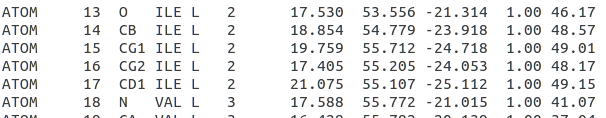
\includegraphics[width=\linewidth]{atom_in_pdb.png}
%}\caption{\small{На снимке экрана показан внешний вид секции ATOM в текстовом редакторе. }}\label{fig:atom_in_pdb}\end{figure}
В настоящий момент известны различные методы для определения пространственной структуры белка. Среди них X-ray кристаллография, электронная микроскопия и ЯМР-спектроскопия~\cite{konf_analiz_belkov}.

База данных структур в формате Protein Data Bank\cite{rcsb} содержит информацию о таких структурах. Поскольку методов много, информацию можно получать разную -- формат файлов в этой базе данных довольно хорошо развит.

PDB файл ~\cite{pdb} содержит информацию о белке, сгруппированную по различным признакам, среди которых нам будут интересны следующие данные: 
\begin{enumerate}
\item Пространственное положение атомов аминокислот (секция ATOM):
включает информацию о координатах каждого из атомов, образующих аминокислоты, в свою очередь образующих цепочки белка или белков, вид атома, другие важные характеристики. Координаты упорядочены по положению аминокислот в цепочке.

\item Информация о вторичной структуре цепочек (секции HELIX, SHEET).
\end{enumerate}


%\newpage\section{Выбор протяженных регионов}
%Для того, чтобы выбрать протяженные регионы для аланинового сканирования, построим итеративный алгоритм.

%Включим в состав множества протяженных регионов, содержащих ,,энергетически горячие аминокислотные остатки'', следующее:
%\begin{itemize}
%\item аминокислоты, образующие ,,интерфейс'' взаимодействия с парной цепочкой или белком (с использованием отсечки по расстоянию от второй цепочки)
%\item аминокислоты, образующие поверхность ,,карманов'', находящихся в области взаимодействия пары белков
%\item не-гидрофобные аминокислоты, являющиеся соседними по отношению к аминокислотам, образующим интерфейс
%\item если интерфейс взаимодействия образован петлями, то добавим все аминокислоты, образующие петли 
%\end{itemize}


%\newpage\subsection{Формализация задачи}
%\begin{frame}{Formal definitions - I}
%\begin{itemize}
%\item Protein molecule - a set of spheres S. Each sphere $s \in S,\,s=s(c_s, r_s)$ has center point $c_s$ and radius $r_s$, ,,atom'' corresponds to sphere.
%\item the Euclidean distance $D(x,\,s)$ 
%of a point $x$ from the surface of a sphere $s$:
%$$
%D(x,\,s) = || x - c_s || - r_s
%$$
%\item The minimal distance from the point x to the nearest sphere (atom) is given by the function r (x):
%$$
%r(x) = \min \{D(x,s) | s \in S \}
%$$
%\end{itemize}
%\end{frame}

\subsection{Маскировка аминокислот}
В качестве предварительной обработки добавим возможность маскировки аминокислот -- исключения из рассмотрения тех фрагментов цепочек, аминокислоты на которых нам не интересны или которые изменять не желательно. 

В качестве примера возьмем случай, когда мы хотим усилить сцепленность между легкой и тяжелой цепями антитела, но при этом не хотим никак повлиять на его специфичность -- в этом случае уместно исключить из рассмотрения CDR-регионы. Противоположная ситуация -- добиться лучшей аффинности с известным антигеном, не нарушив при этом структуру FR-регионов антитела.

Маскируемые регионы в приведенных примерах могут быть получены, например, в результате алгоритма аннотирования, приведенного в работе \cite{yakovlev2014}.

%\todo{или идея в том, что мы не рассматриваем CDR потому что они гипервариабельные, и изменить одну амк на них технически нереально?}
%Исходя
\subsection{Триангуляция Делоне}
Рассмотрим объединение сфер $S$, каждая из которых (обозначим ее $s$) характеризуется координатами своего центра $c_s=(x_s, y_s, z_s)$ в трехмерном пространстве и радиусом $r_s$:
$$
s=s(c_s,\,r_s),\quad s\in S.
$$
Каждому атому цепочки белка будем сопоставлять такую сферу с координатами центра, совпадающими с координатами атома в PDB-файле, и радиусом, соответствующим радиусу Ван-дер-Ваальса для данного атома, про все атомы цепочки будем говорить, что вместе они образуют такое объединение сфер.

Для определенности далее будем обозначать $S_1$ -- объединение сфер, соответствующее цепочке, на которой осуществляется поиск региона, определяющего специфичность, $S_2$ -- объединение сфер, соответствующее цепочке, образующей комплекс совместно с цепочкой $S_1$ и по отношению к которой специфичен построенный регион. 

Но каким образом перейти от дискретного множества точек в пространстве (или в нашем случае -- от множества сфер $S$) к поверхности? Для этого ,,достраивают'' множество таких дискретных объектов с помощью триангуляции Делоне (в трехмерном случае также  корректно называть ее тетраэдризацией, при обобщении на пространства размерности 3 и выше ее также называют тесселяцией), в результате чего пространство разбивается на тетраэдры с вершинами в точках множества $S$, такие, что любые два из них могут в пересечении иметь только одно из ребер, одну из граней или одну из вершин, или не иметь общих точек, при этом их объединение образует выпуклый многогранник.

%Диаграмма Вороного конечного множества точек S на плоскости представляет такое разбиение плоскости, при котором каждая область этого разбиения образует множество точек, более близких к одному из элементов множества $S$, чем к любому другому элементу множества. Двойственная


Используя Евклидово расстояние между парой точек с известными координатами в прямоугольной декартовой системе координат $p_1=(x_1, y_1, z_1)$ и $p_2=(x_2, y_2, z_2)$, которое определено формулой:
$$d(p_1, p_2) =\sqrt{(x_1-x_2)^2+(y_1-y_2)^2+(z_1-z_2)^2}, $$ 
определяют условие, которое должно выполняться для всех тетраэдров, вместе образующих тетраэдризацию Делоне -- так называемый критерий (условие) Делоне: сфера, описанная около такого тетраэдра, не должна содержать внутри никакие точки множества $S$, но при этом точки множества $S$ могут находиться на сфере.

Проверку выполнения условия Делоне для точек в трехмерном пространстве также проводят с помощью вычисления знака определителя \cite{delaunay_tesselations}:
\begin{equation}
InSphere(a, b, c, d; p) = \left|
\begin{array}{ccccc}
a_1 & a_x & a_y & a_z & a_q \\ 
b_1 & b_x & b_y & b_z & b_q  \\ 
c_1 & c_x & c_y & c_z & c_q \\ 
d_1 & d_x & d_y & d_z & d_q \\ 
p_1 & p_x & p_y & p_z & p_q 
\end{array} \right|,\label{ch2:det}
\end{equation}
 
в котором произвольной точке $p=(p_x, p_y, p_z)$ -- с известными декартовыми координатами $p_x$, $p_y$, $p_z$ в трехмерном пространстве сопоставлен кортеж 
\begin{equation}
p=(p_1,\,p_x,\, p_y,\, p_z,\,p_q), \label{ch2:f1}
\end{equation}
такой, что
$$
p_q=p_x^2+p_y^2+p_z^2,
$$ 
$p_1$ -- обобщенная координата, которая равна $1$ для всех точек, за исключением особой точки ,,в бесконечности'', кортеж для которой имеет вид ${\infty=(0,0,0,0,1)}$; точки $a, b, c, d$ -- задают вершины тетраэдра, для которого проверяется условие Делоне, а точка $p$ -- точка, для которой проверяется положение относительно описанной около тетраэдра сферы. 

В настоящей работе для построения тетраэдризации Делоне для данного множества точек используется готовая реализация из пакета QHull \cite{qhull} (обертка для этого пакета на языке  python из библиотеки SciPy~\cite{scipy}), алгоритм которой основан на построении выпуклой оболочки для множества точек в пространстве большей размерности, переход к которому осуществляется с помощью сопоставления координатам в трехмерном пространстве  кортежей (\ref{ch2:f1}), а критерий Делоне проверяется с помощью приведенного выше определителя (\ref{ch2:det}). 



%\begin{frame}{Formal definitions - I}
%\begin{itemize}
%\item Protein molecule - a set of spheres S. Each sphere $s \in S,\,s=s(c_s, r_s)$ has center point $c_s$ and radius $r_s$, ,,atom'' corresponds to sphere.
%\item the Euclidean distance $D(x,\,s)$ 
%of a point $x$ from the surface of a sphere $s$:
%$$
%D(x,\,s) = || x - c_s || - r_s
%$$
%\item The minimal distance from the point x to the nearest sphere (atom) is given by the function r (x):
%$$
%r(x) = \min \{D(x,s) | s \in S \}
%$$
%\end{itemize}
%\end{frame}\newpage
\subsection{Построение двойственного графа}
Имея в своем распоряжении объединение сфер $S$, сопоставленное атомам, образующим цепочку белка, умея сопоставлять этому объединению поверхность и находить с помощью нее соседние сферы, можно быстрее проводить дальнейший анализ. Например, найти все сферы, образующие внешнюю границу молекулярной поверхности или ее фрагмент.

Для этого можно использовать разные подходы. Например, определить множество близко расположенных сфер, образующих нерв, воспользовавшись алгоритмом Эдельсбруннера \cite{alpha_shapes1995, alpha_shapes1998}, затем по объектам, находящихся на его внешней границе, построить молекулярную поверхность или определить карманы (как объединения тетраэдров, отбракованных алгоритмом). Другой подход, который будем использовать для построения алгоритма мы, предполагает построение двойственного по отношению к тетраэдризации Делоне графа и поиск в ширину в этом графе. Вместо поиска в ширину может использоваться, например, алгоритм Дейкстры с какой-либо модификацией \cite{caver2007}.

Мы будем строить двойственный граф по тому же принципу, по которому это сделано в работе \cite{caver2007}. Вершинам графа сопоставим треугольники тетраэдризации Делоне, а ребра между вершинами будем проводить по принципу,  %проиллюстрированному на рисунке \ref{fig:tetra} и 
описанному далее. 

Вспомним, что вершинам тетраэдров соответствуют координаты центров атомов с известными радиусами Ван-дер-Ваальса, то есть поместим в вершины тетраэдра центры сфер с различными радиусами $r_1$, $r_2$, $r_3$, $r_4$.

Рассмотрим сферу фиксированного радиуса $r$. Представим, при каких условиях она может пересечь одну из граней тетраэдра, и частично оказаться внутри него -- так, чтобы при этом не пересечь ни одну из сфер, построенных в  вершинах тетраэдра. 

Построим для такой грани-треугольника окружность так, чтобы она касалась окружностей, образованных пересечением сфер, построенных в вершинах, с плоскостью, в которой лежит треугольник. Если радиус такой окружности не меньше, чем $r$, то сфера фиксированного радиуса сможет пройти через нее так, чтобы не нарушить поставленное условие.

При выполнении такого условия для одной из граней тетраэдра каждой паре граней-треугольников сопоставим ребро.

В работе \cite{caver2007} используется более простое, более грубое, но легче проверяемое условие ,,проходимости'' между гранями тетраэдров: в ней сфера радиуса $r$ может проходить только по ребру, общему для двух граней. 

В нашем случае условие нужно для того, чтобы  ребра позволяли достичь всех треугольников, содержащих атомы, которых может касаться сфера радиуса $r$. 
%\begin{itemize}
%\item Рассматриваем одновременно 2 цепочки, образующие белковый комплекс.
%\item Начнем с построения выпуклой оболочки и триангуляции Делоне для каждой из них, будем искать протяженные регионы с энергетически горячими аминокислотными остатками  на одной из них. Строить будем по центрам атомов, формирующих аминокислоты цепочки.
%\item Выберем все треугольники выпуклой оболочки, в которых хотя бы одна вершина удалена от некоторых атомов второй цепочки не далее, чем на выбранное (фиксированное) значение отсечки.
%\end{itemize}


%\begin{itemize}
%\item Берется структура в PDB.
%\item Центры атомов рассматриваются как точки. По ним строится триангуляция Делоне (с помощью scipy.delaunay - обертки над алгоритмом qhull).
%\item Берется невзвешенная триангуляция -- по тем же соображениям, по которым она используется в CAVER (эвристика)\cite{caver2007}.
%\end{itemize}
%Я сопоставляю графу триангуляцию по тому же принципу, как в статье по CAVER:


%\begin{figure}[h]
%\resizebox{!}{0.3\textheight}{
%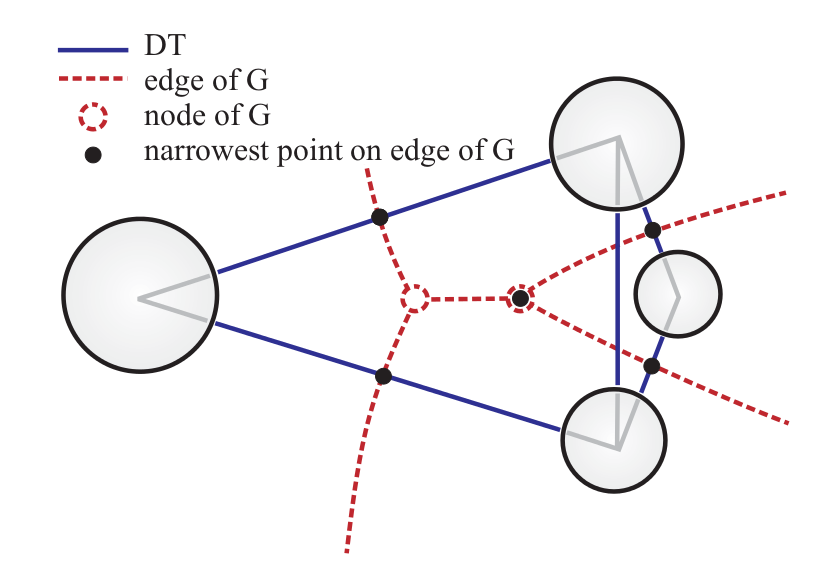
\includegraphics{image4_caver.png}
%}

%\caption{\small{[Computation of tunnels in protein molecules using
%Delaunay triangulation, P.Medek, et al., 2007]
% }}
%\label{fig:image4_caver}
%\end{figure}

%Треугольники триангуляции -- вершины графа, ребра графа -- общие стороны треугольников (с ограничением снизу на длину).

%Дополнительно используется такой же граф по треугольникам выпуклой оболочки (без ограничения снизу на длину стороны, просто по смежным по стороне треугольникам).

%Выбирается начальное множество треугольников выпуклой оболочки. Сейчас берутся треугольники, вершины которых недалеко (в смысле отсечки по расстоянию) от второго белка.

%\newpage
\subsection{Выбор начального множества треугольников}

Будем исходить из предположения о том, что специфичность определяется в первую очередь интерфейсом взаимодействия, поэтому будем начинать строить регион, определяющий специфичность взаимодействующих цепочек, от области интерфейса взаимодействия.

Итак, в нашем распоряжении тетраэдризация Делоне, внешняя граница которой представляет собой выпуклый многогранник, а также граф, позволяющий перемещаться между треугольниками тетраэдризации.

Можно предложить несколько стратегий для выбора начального множества треугольников:
\begin{enumerate}
\item Параметризовав выбор с помощью числовой характеристики -- величины отсечки, будем выбирать те вершины выпуклой оболочки тетраэдризации Делоне, которые удалены от атомов второй цепочки не далее, чем на выбранную величину. В качестве начального множества выберем все треугольники выпуклой оболочки, которые содержат хотя бы одну такую вершину.
\item Используя параметр -- величину отсечки, выберем начальное множество атомов, удаленных не более, чем на величину отсечки от атомов второй цепочки. В качестве начального множества треугольников выберем треугольники выпуклой оболочки, в вершинах которых лежат какие-либо из выбранных атомов.  
\item Объединим множества атомов цепочек $S_1$ и $S_2$, построим тетраэдризацию Делоне по их объединению. Среди полученной тетраэдризации выберем в качестве начального множества треугольники, которые являются гранями тетраэдров, построенных на атомах из $S_1$ и $S_2$, и при этом таких, что все образующие их вершины принадлежат $S_1$. Затем удалим из тетраэдризации все вершины, которые принадлежали $S_2$, вместе с соответствующими гранями и ребрами, в результате на оставшемся множестве тетраэдров по-прежнему будет выполняться критерий Делоне, при этом тетраэдризация может перестать быть выпуклой.
\end{enumerate} 

В работе реализована первая стратегия, как наиболее простая и предполагающая выбор минимального множества атомов на первом этапе. Третья стратегия может дать лучшие результаты в случае, если интерфейс белок-белкового взаимодействия образован областью комплиментарного кармана. 

%Включим в состав множества протяженных регионов, содержащих ,,энергетически горячие аминокислотные остатки'', следующее: аминокислоты, образующие ,,интерфейс'' взаимодействия с парной цепочкой или белком (с использованием отсечки по расстоянию от второй цепочки)
%\todo{вспомнить, что я хотела сказать таким заголовком}
%\begin{itemize}
%\item определяем множество треугольников выпуклой оболочки, для которых хотя бы одна вершина удалена от центров атомов второй цепочки не больше, чем на выбранное значение отсечки
%\item Далее расширяем интерфейс
%\begin{itemize}
%\item шаг 1: добавляем к интерфейсу все треугольники выпуклой оболочки, содержащие атомы аминокислот, которые уже туда попали
%\item шаг 2: продлеваем регион до границы гидрофобности
%\item шаг 3: продлеваем регион за границы гидрофобности на 1 аминокислоту.
%\end{itemize}
%\end{itemize}


В результате выбора одной из стратегий получаем одну или несколько протяженных связных областей -- треугольников выпуклой оболочки -- по которым можно восстановить позиции аминокислот или найти близко расположенные карманы.

%\newpage
\subsection{Поиск карманов}
%\todo{переписать}
Поиск карманов, каналов и полостей в макромолекулах является хорошо изученной задачей \cite{alpha_shapes1995, alpha_shapes1998, caver2007, ppi_kim2006}. Существуют сервисы на основе этих статей, которые выполняют поиск молекулярных карманов для конкретной структуры~\cite{castp}. 

С помощью поиска в ширину по двойственному графу, начиная с треугольников, выбранных на предыдущем этапе, выберем все пройденные таким образом треугольники.

Дополнительно нам потребуется убедиться, что выбранные при поиске карманов треугольники-грани тетраэдров не удалены от области интерфейса и выбранных в качестве первого приближения треугольников слишком далеко (например, карман может выходить на внешнюю поверхность с другой стороны, то есть оказаться сквозным каналом или порой), для этого добавим дополнительную эвристику: будем переходить в следующий треугольник по ребру только в том случае, если он ближе к одной из вершин какого-либо из выбранных на предыдущем шаге треугольников, чем к их ,,не выбранным'' соседям.

%\begin{itemize}
%\item Начинаем с множества отобранных треугольников выпуклой оболочки (черным цветом)
%\item Ищем в ширину с ограничениями
%\item Ходим только по тем треугольникам, для которых ближайший треугольник выпуклой оболочки -- один из отобранных треугольников выпуклой оболочки, а не какой-либо из других треугольников выпуклой оболочки.
%\item Ближайший треугольник == в смысле расстояния до ближайшей из вершин он ближе, чем другие треугольники выпуклой оболочки
%\end{itemize}
%\cite{alpha_shapes1995, alpha_shapes1998}
%\newpage
\subsection{Расширение интерфейса. Добавление петель}

Перед добавлением петель треугольники тетраэдризации, которые были выбраны на предыдущих шагах, преобразуются в фрагменты последовательности аминокислот. Для этого по каждой из вершин, образующих треугольник, восстанавливается информация об атоме, по ней -- информация о позиции аминокислоты, к которой он принадлежит. Затем происходит удаление дублей.

Получив таким образом список позиций аминокислот, продлеваем их, используя информацию о вторичной структуре.

Вторичная структура определяется на основе вывода DSSP \footnote{используется обертка к DSSP в составе пакета biopython}.

Рассматриваются позиции аминокислот, образующих непрерывные фрагменты структуры, которые не определяются как $\alpha$-спирали или $\beta$-листы, среди них выбираются те, в состав которых попадает какая-либо из позиций аминокислот, уже выбранных в состав региона, определяющего специфичность, и целиком добавляются к выделяемому региону.

%\todo{\item Я беру непрерывные фрагменты структуры, которые не определяются как альфа-спирали или бета-листы, выбираю среди них те, в которые попадает какая-либо аминокислота, ну и добавляю их к выделяемому контуру - технической сложности никакой.}




%\begin{itemize}


%\todo{\item вариантов 2: либо не добавлять петли целиком, вместо этого добавлять только такие фрагменты (в статье они приведены), либо как-то их отмечать на выделенных петлях + отмечать на удаленных петлях, которые в выделенный регион не попали.}

% \todo{\item про HMM думаю, напишу через пару дней.}

% \todo{\item вообще если получится, я разберусь как считать взвешенную триангуляцию Делоне и с помощью нее искать карманы.}


%\end{itemize}

\section{Программная реализация}

Алгоритм поиска протяженных регионов, определяющих специфичность, реализован на языке python, с применением библиотек SciPy\cite{scipy} и NumPy\cite{numpy}.

Кроме того, написан плагин для приложения PyMOL~\cite{pymol}, визуализирующий регион, определяющий специфичность, для выбранной структуры.

Исходный код примеров, скриптов и плагина доступен в git-репозитории \url{https://github.com/latticetower/MS_thesis}.

Алгоритм не учитывает ситуации, когда энергетический значимой является удаленная от интерфейса взаимодействия аминокислота, находящаяся на подвижном фрагменте цепочки и влияющая на взаимодействие комплекса косвенно. Энергетическая значимость в таких случаях достигается за счет изменения поворотов боковых цепей близко расположенных в пространстве аминокислот, что может привести к изменению поворота боковой цепи аминокислоты, расположенной вблизи интерфейса белок-белкового взаимодействия и привести к изменению сцепленности цепочек комплекса (можно представить каскад петель, для которого точечная мутация одной аминокислоты на одной из петель приводит к повороту всех петель).

К сожалению, принципы, по которым можно выявлять такие аминокислоты, не ясны, поэтому в настоящей работе алгоритмом поиска  регионов, определяющих специфичность, они не учитываются.